\documentclass[./einleitung.tex]{subfiles}
\usepackage{float}
\usepackage{float}
\usepackage{float}
\usepackage{float}
\usepackage{natbib}
\begin{document}
    \section{Die Nutzung des \acrshort{lsp}}
    \subsection{Installationsmöglichkeiten}
    Der \acrshort{lsp}-Server benötigt keine zusätzlichen Strukturen und kann direkt als Datei ausgeführt werden.
    Deshalb ist die normale Vorgehensweise das Ablegen des \acrshort{lsp}-Servers in einem Zentralen Server und das Hinzufügen des Pfades zu dem Umgebungsvariablen.
    Im Beispiel wurde die Datei zu `dmflsp' umbenannt, damit der Name genauer das Programm beschreibt und nicht mit anderen \acrshort{lsp}-Server kollidieren kann.\\
    \begin{figure}[h]
        \centering
        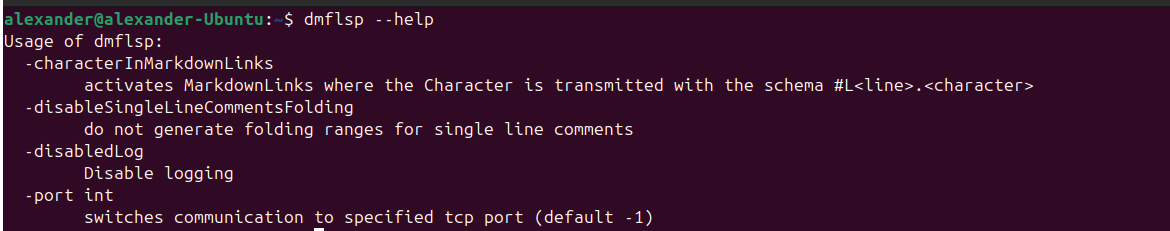
\includegraphics[width=\linewidth]{bilder/screenshot-lsp-help}
        \caption{Aufruf des \acrshort{cli} des \acrshort{lsp}-Servers}
        \label{fig:screenshot-lsp-help}
    \end{figure}\\
    Es gibt Editoren die eine native Anbindung eines \acrshort{lsp}-Servers ermöglichen.
        {\footnotesize TODO Zed Besspiel }
    \subsubsection{Intellij}
    Intellij unterstützt nur wenige \acrshort{lsp}-Funktionen ohne zusätzliche Plugins.
    Mit von `lsp4ij' können \acrshort{lsp}-Server direkt in der Oberfläche konfiguriert werden.\\
    \begin{figure}[h]
        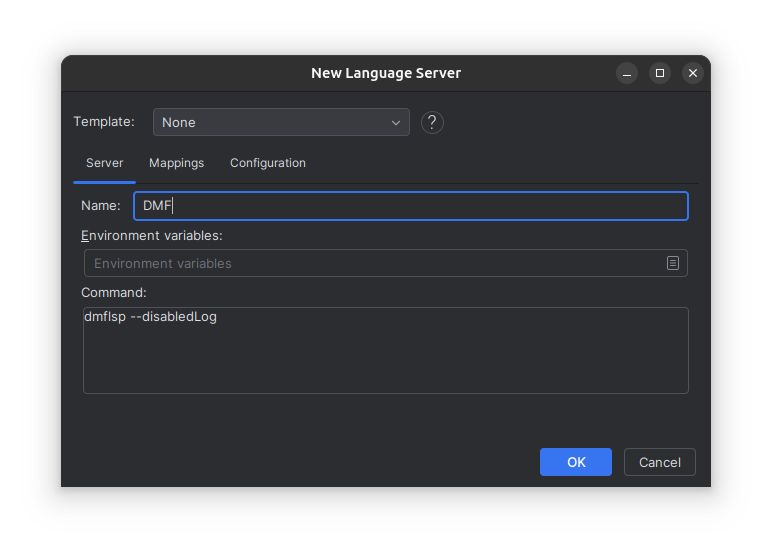
\includegraphics[width=\linewidth / 2]{bilder/screenshot-add-lsp-lsp4ij}
        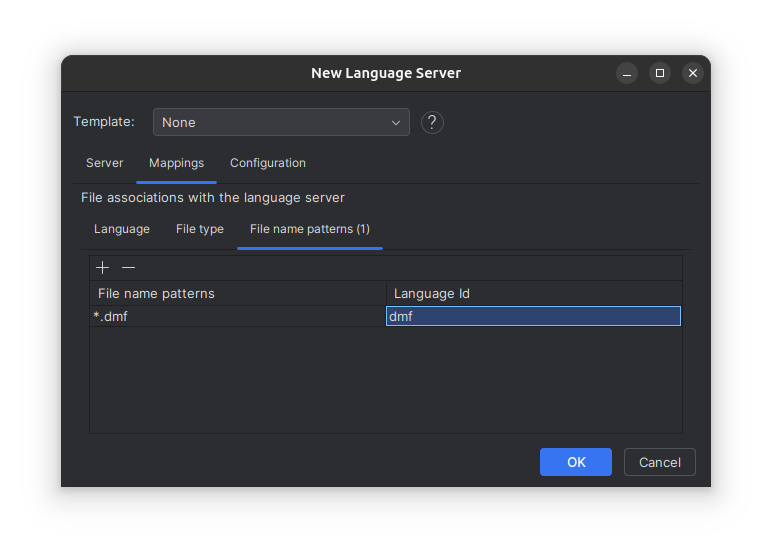
\includegraphics[width=\linewidth / 2]{bilder/screenshot-file-mapping}
        \caption{lsp4ij Konfiguration}
        \label{fig:screenshot-add-lsp-lsp4ij}
    \end{figure}\\
    Um diese Konfiguration automatisch anzulegen und den Dateien ein passendes Icon zu geben, kann das Intellij-Plugin für das \acrshort{dmf} verwendet werden.
    Es enthält die verschiedenen Versionen des Servers und kann sie automatisch an den konfigurierten Pfad ablegen.
    Der Pfad zum \acrshort{lsp}-Server kann entweder in den Einstellungen des Plugins oder über die Umgebungsvariable `DMF\_LSP' konfiguriert werden.

    \subsubsection{Visual Studio Code}
    Um den \acrshort{lsp}-Server in Visual Studio Code nutzen zu können, wird die Erweiterung für das \acrshort{dmf} benötigt.
    Dieses enthält die Logik zum Verbinden zum Server und die verschiedenen Versionen.
    Die benötigte Version kann direkt ausgeführt werden und benötigt keine zusätzliche Konfiguration.\\
    Im Gegensatz zu den bisherigen Konfigurationen nutzt die Visual Studio Code Erweiterung eine \acrshort{tcp}-Verbindung.


    \subsection{Funktionen im Editor}
    Während des Bearbeitens der Modelle können die Funktionen des \acrshort{lsp}-Servers genutzt werden.
    In diesem Abschnitt werden die Funktionen präsentiert.
    
    \subsubsection{Einfärbung des Textes}
    Mithilfe der semantischen Token kann der Editor den Text der Modelldatei einfärben.
    Da der Server nicht die Farbe, sondern nur die Funktion, vorgibt, wird der Text anhand der Einstellungen der Entwickler*innen eingefärbt.
    \begin{figure}[H]
        \centering
        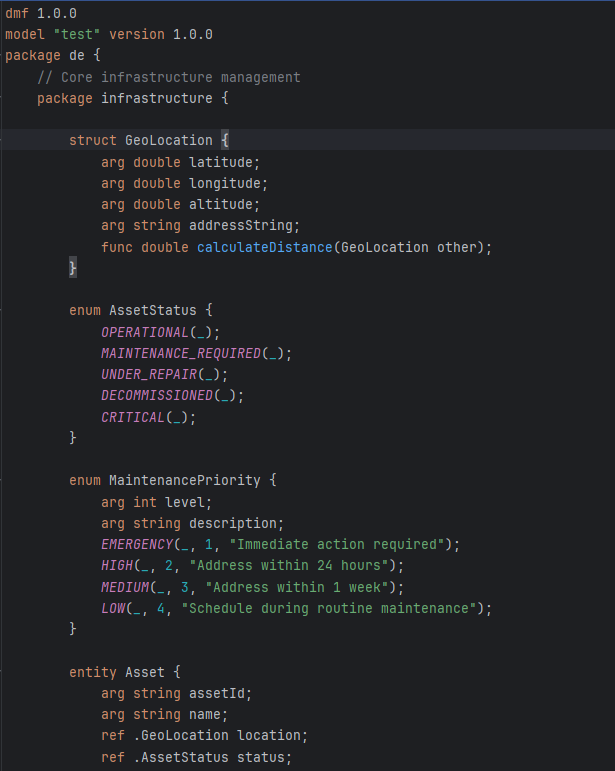
\includegraphics[width=\linewidth / 2 - 1em]{bilder/semanticIntellij}
        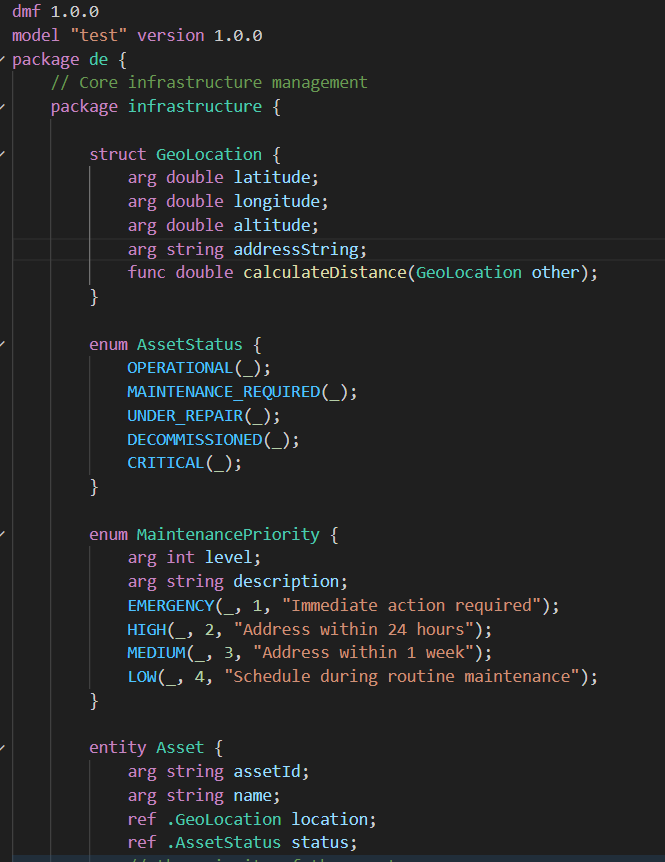
\includegraphics[width=\linewidth / 2 - 1em]{bilder/semanticVscode}
        \caption{Eingefärbte Modelldateien in Intellij und Visual Studio Code}
        \label{fig:semanticintellij}
    \end{figure}

    \subsubsection{Diagnosen}
    Wenn der Fehler in der Datei existieren werden diese automatisch im Editor markiert.
    Es wird auch eine Beschreibung und die detaillierte Beschreibung, welche auch im Generator ausgegeben wird, übertragen.\\
    Die Darstellung wird von der \acrshort{ide} übernommen.
    In Intellij und Visual Studio Code wird die Hover-Beschreibung zusätzlich angezeigt.\\
    \begin{figure}[hH]
        \centering
        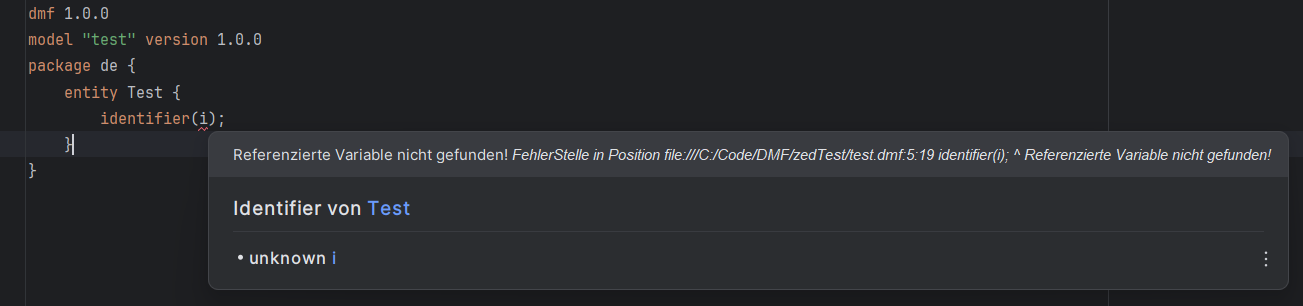
\includegraphics[keepaspectratio,height=8em]{bilder/markierung-fehler-intellij}
        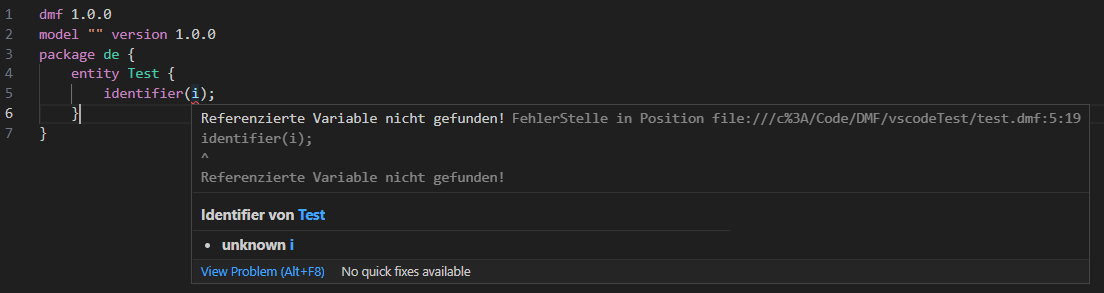
\includegraphics[keepaspectratio,height=8em]{bilder/markierung-fehler-vscode}
        \caption{Beispiele aus Intellij und Visual Studio Code}
        \label{fig:markierung-fehler-intellij}
    \end{figure}

    \subsubsection{Hover-Beschreibungen}
    Um Informationen über ein Element bereitzustellen, kann mit dem Mauszeiger über einem Element gehovered werden.
    Für alle PackageElemente, EntityIdentifier, Argumente, Referenzen, MultiReferenzen und Kommentare können Beschreibungen angezeigt werden.
    Mithilfe von Links in den Beschreibungen kann direkt zum erwähnten Element navigiert werden.
    \begin{figure}[H]
        \centering
        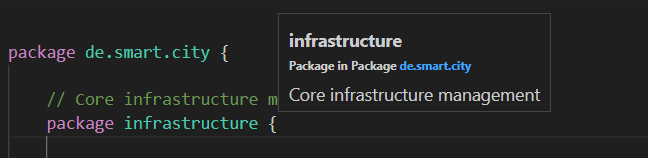
\includegraphics[height=5em]{bilder/hover-package}
        \caption{Beschreibung eines Package Elements}
        \label{fig:hover-package}
    \end{figure}
    Bei PackageElementen enthält die Beschreibung den Kommentar des Elements sowie das Package, in dem es liegt.
    \begin{figure}[H]
        \centering
        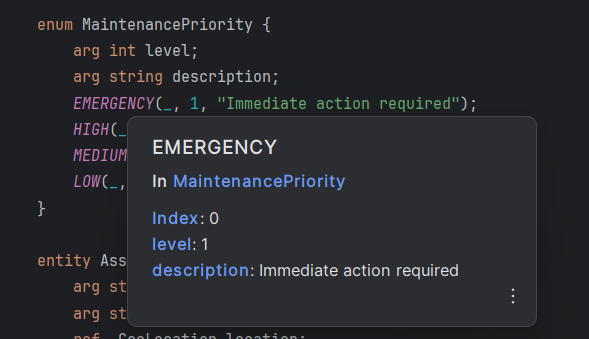
\includegraphics[height=7em]{bilder/hover-enum-entry}
        \caption{Beschreibung einer Enum Konstante ohne Kommentar}
        \label{fig:hover-enum-entry}
    \end{figure}
    Die Beschreibung von Enum Konstanten enthält das Enum, falls vorhanden den Kommentar und die Argumente des Enum mit den Werten der Konstante.
    Der erste Wert ist der Index, welcher in der Datenbank gespeichert wird.
    \begin{figure}[H]
        \centering
        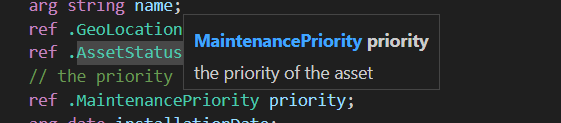
\includegraphics[height=5em]{bilder/hover-referenz}
        \caption{Beschreibung einer Referenz}
        \label{fig:hover-referenzen}
    \end{figure}
    Referenzen enthalten den Kommentar sowie den Typen und Namen der Variable.
    Argumente und MultiReferenzen verhalten sich gleich.
    \begin{figure}[H]
        \centering
        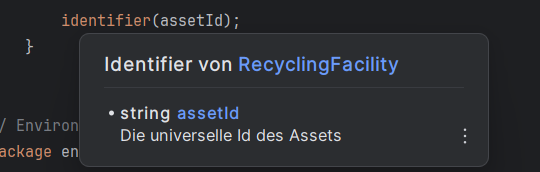
\includegraphics[height=7em]{bilder/hover-entity-identifier}
        \caption{Beschreibung eines Entity Identifiers}
        \label{fig:hover-entity-identifier}
    \end{figure}
    Bei einem Entity Identifier werden die referenzierten Variablen ihren Kommentaren angezeigt.

    \subsubsection{Referenzen}
    In den \acrshort{ide}s können die Referenzen aufgerufen werden.
    Der \acrshort{dmf}-\acrshort{lsp}-Server findet Referenzen, Deklarationen und Verwendungen in Parametern und EntityIdentifier.
    \begin{figure}[H]
        \centering
        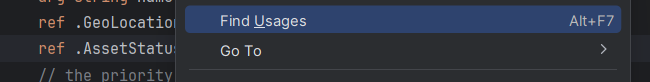
\includegraphics[height=2.5em]{bilder/callReferencen}
        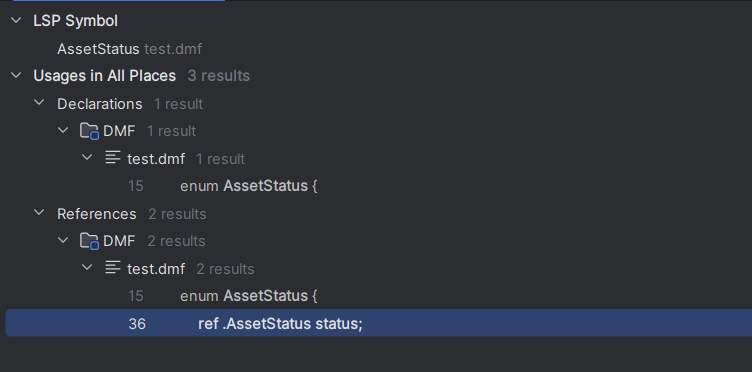
\includegraphics[height=6em]{bilder/referencen}
        \caption{Aufruf der Referenzen}
        \label{fig:callreferencen}
    \end{figure}

    \subsubsection{Faltbereiche}
    Damit Entwickler*innen in großen Dateien die Übersicht behalten können unterstützt der \acrshort{lsp}-Server die Übermittlung von Faltbereichen.
    Die Steuerung der Faltbereiche ist \acrshort{ide} spezifisch.
    \begin{figure}[H]
        \centering
        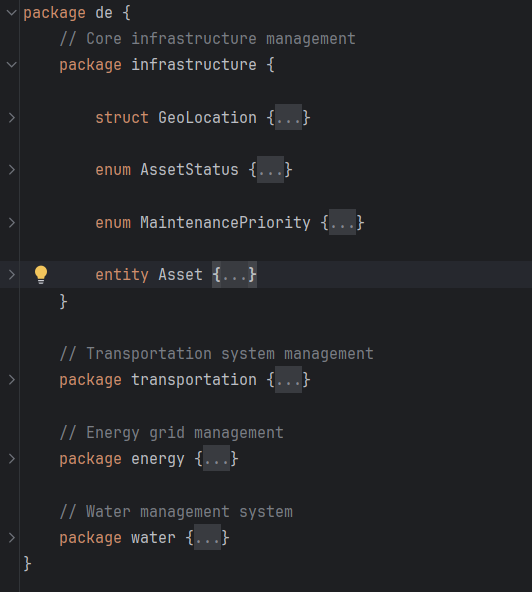
\includegraphics[height=15em]{bilder/faltbereich}
        \caption{Nutzung der Faltbereiche}
        \label{fig:faltbereich}
    \end{figure}

    \subsubsection{Auswahlbereiche}
    Damit die Entwickler*innen auch verschiedene Elemente gut Auswählen können, werden die Auswahlbereiche von \acrshort{lsp}-Server berechnet.
    \begin{figure}[H]
        \centering
        $\vimage{bilder/selection1.png}\vpointer
        \vimage{bilder/selection2.png}\vpointer
        \vimage{bilder/selection3.png}\vpointer
        \vimage{bilder/selection4.png}\vpointer
        \vimage{bilder/selection5.png}$
        \caption{Nutzung der Auswahlbereiche}
        \label{fig:selection}
    \end{figure}

    \section{Nutzung des \acrshort{dmf}}\label{sec:nutzung-des-dmf}
    Zum Darstellen der Benutzung des \acrshort{dmf} wird das Anlegen eines Projektes mit einem Java und einen Typescript Programm beschrieben.

    \begin{figure}[H]
        \caption{Dateiaufbau für ein Beispielprojekt}
        \dirtree{%
            .0 .
            .1 Modell.
            .2 domain.dmf.
            .1 TSProjekt.
            .2 src.
            .3 domain (Modell).
            .3 delegates (Delegates).
            .3 projekt (Projekt).
            .1 JDomain.
            .2 src/gen/java (Modell).
            .2 src/main/java (Delegates).
            .1 JProjekt.
            .2 src/main/java (Projekt).
        }
        \label{fig:dirtree}
    \end{figure}

    \paragraph{Im Modell} Ordner wird das Modell abgelegt.
    Die Bereitstellung kann an die Organisation angepasst werden, da die restlichen Projekte per relativen Pfad auf die Datei zugreifen.
    Entscheidend ist dabei die Organisation der Git Repositories.
    Werden die verschiedenen Komponenten (Modell, Typescript Projekt, Java Projekt) in verschiedenen Repositories abgelegt, so handelt es sich um eine Poly-Repository Struktur. \cite{monorepo}
    Die Verwaltung der verschiedenen Repositories kann manuell durch Entwickler*innen oder durch Build Scripte gesteuert werden.
    Konträr zur Poly-Repository Struktur ist die Mono-Repository Struktur.
    Bei dieser werden alle Projekte in einem Repository verwaltet. \cite{monorepo}
    Hier entfällt die Synchronisation des Modells.

    \paragraph{Das Typescript Projekt} enthält sowohl die generierten Dateien als auch den Source Code des eigentlichen Projekts.
    Dies kann besonders in kleinen Projekten den Aufwand reduzieren.

    \paragraph{Das Java Projekt} wird in mehrere Artefakte unterteilt.
    Dies dient der Strukturierung von größeren Projekten und wurde exemplarisch genutzt, obwohl das Beispiel Projekt nur ein weiteres Artefakt besitzt.
    Innerhalb des JDomain Artefakts werden Modell und Delegates in verschiedene Ordner generiert, damit nur die Delegates von der Versionsverwaltung beachtet werden können und \acrshort{ide}s die Dateien richtig verwalten können.

    \subsection{Anlage des Typescript Projektes}\label{subsec:anlage-des-typescript-projektes}
    Das Beispiel Typescript Projekt nutzt die Bibliothek `Express' um einen kleinen Webserver zu implementieren.
    Ziel ist es die Verwendung des \acrshort{dmf} im Kontext einer simplen Restschnittstelle zu zeigen.\\
    Das Projekt wurde mithilfe der einer Anleitung von \citeauthor{initExpress} angelegt.\\
    Zuerst wird die `package.json'-Datei mithilfe der NPM-\acrshort{cli} angelegt.
    In ihr wird das Projekt beschrieben.
    Dazu gehören unter anderem der Name, Version, Abhängigkeiten und Ausführungskonfigurationen.\\
    Zu den Abhängigkeiten werden Dotenv, Typescript und Express hinzugefügt.
    Die Abhängigkeiten zu den Typen von Typescript und Express werden als `DevDependecies' hinzugefügt.
    So werden sie nur während der Entwicklung genutzt.\\
    Der nächste Schritt der Einrichtung ist die Konfiguration von Typescript.
    Es werden die Ordner für Source Code und Output sowie die beabsichtigte Version des JavaScript-Standards angegeben.\\
    Nun kann die Beispielimplementierung aus der Anleitung angelegt werden.
    Diese kann mit folgendem Befehl ausgeführt werden.
    \begin{lstlisting}{language=bash, caption=Start description Servers, label=lst:startExpress}
npx ts-node src/index.ts
    \end{lstlisting}
    Kann der Server aufgerufen werden, war die bisherige Anlage erfolgreich.
    Als nächstes kann das \acrshort{dmf} hinzugefügt werden.
    Dafür werden die Ausführungskonfigurationen erweitert.
    \begin{lstlisting}[language=json, caption=Ausführungskonfigurationen in package.json, label=lst:packageScripts]
"scripts": {
    "run": "npx ts-node src/index.ts",
    "build": "npm run generateModell && npm run generateDelegates && npx tsc",
    "start": "node dist/index.js",
    "generateModell": "generator --basePath ./src --mode ts --modelFile ../Modell/domain.dmf",
    "generateDelegates": "generator --basePath ./src --mode tsDelegates --modelFile ../Modell/domain.dmf",
  },
    \end{lstlisting}
    Es werden zwei neue Konfigurationen hinzugefügt: generateModell und generateDelegates.
    Sie rufen den Generator mit den Parametern für den Source Code Ordner, dem Pfad der Modelldatei und dem jeweiligen Generationsziel auf.
    Da die Konfigurationen in der Build Konfiguration eingebaut wurden, werden sie bei jedem Build automatisch ausgeführt.
    \paragraph{Die generierten Modelldateien} werden in den Ordnern nach ihrem Package Pfad abgelegt.
    Im Beispiel wird die Entität User genutzt.
    \begin{lstlisting}[language=Typescript,caption=User.ts, label=lst:userTs]
import * as delegate from "../delegates/domain/UserDelegate";

export class User {
    id: number;
    name: string;

    constructor(id: number, name: string) {
        this.id = id;
        this.name = name;
    }

    sayName(): string {
        return delegate.sayName(this);
    }
}
    \end{lstlisting} % TODO Beispiele für mehr Elemente
    In der Modellklasse sind alle Variablen und Funktionen enthalten.
    Die Delegate Funktionen werden importiert und in den Funktionen der Modellklasse aufgerufen.
    \begin{lstlisting}[language=Typescript, caption=UserDelegate.ts, label=lst:userDelegateTs]
import { User } from "../../domain/User";

export function sayName(caller: User): string {
    return "My Name is "+caller.name;
}
    \end{lstlisting}
    In der Delegatedatei werden die Funktionen mti dem zusätzlichen Caller generiert.
    Die Inhalte der Funktionen müssen die Entwickler*innen selbstständig implementieren.
    \\\\
    Im Server kann nun ein neuer Endpunkt hinzugefügt werden, welcher eine Instanz des Users erstellt und ausgibt.
    In einem realen Projekt würden an dieser Stelle die Prozesse des Programms mit den modellierten Elementen aufgerufen werden.
    \begin{lstlisting}[language=Typescript, caption=Neuer Endpunkt in index.ts, label=indexTs]
app.get("/user", (req: Request, res: Response) => {
    let user: User = new User(1, "Test")
    res.send(user);
});
    \end{lstlisting}

    \subsection{Anlage des Java Projektes}\label{subsec:anlage-des-java-projektes}
\end{document}